\documentclass[../main.tex]{subfiles}
Die Vielzahl an vorhandenen Festungen der Schweiz stellten wir auf einer Karte dar. Den Fokus setzten wir dabei auf grosse oder strategisch wichtige Festungen.

Eine der grössten war die Festung St. Maurice. Mit ihrer Positionierung wäre sie für das Abwehren sämtlicher Angriffe von Westen mitverantwortlich gewesen. Sie bestand aus mehreren einzelnen Festungen, die teilweise miteinander verbunden waren. Der Aufbau unterscheidet sich nicht massgeblich von dem, was wir bei unserer Führung durch die Festung Vitznau entdeckten. 

\begin{figure}[h]
    \centering
    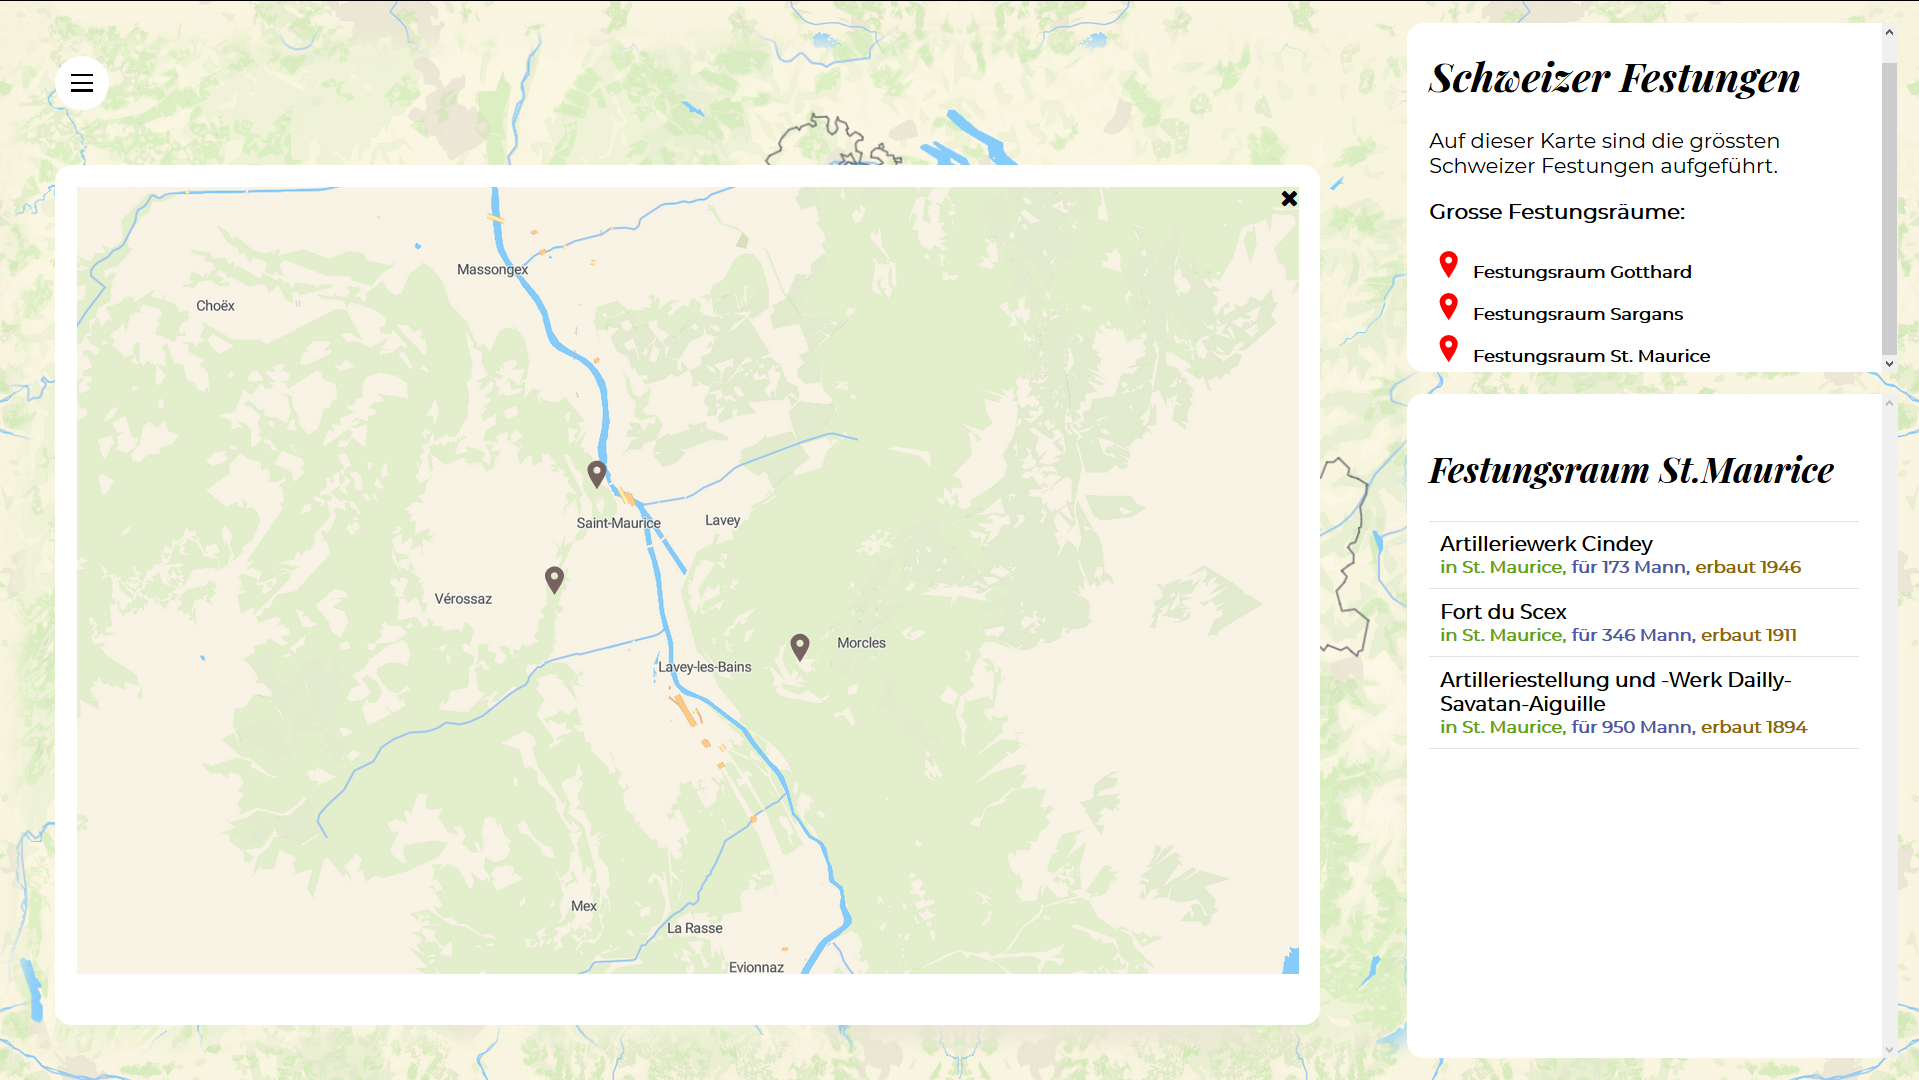
\includegraphics[width=\textwidth,height=7cm,keepaspectratio]{images/screenshot-produkt.png}
    \caption[{Screenshot unserer Webseite (2019). Eine wehrhafte Schweiz. (21. August 2019). \newline URL: https://eine-wehrhafte-schweiz.kairos-solutions.ch/karte/festungen [Stand 24.08.2019] }] {Screenshot unserer Webseite}
\end{figure}

Unser finales Produkt beinhaltet eine Karte, welche einen Überblick über die Schweiz und deren Bunker verschafft. Die Spezifikationen der Bunker sind der Karte ebenfalls zu entnehmen.